\documentclass[12pt, specialist, subf, substylefile = spbu.rtx]{disser}
\usepackage[a4paper, includefoot,
            left=3cm, right=1.5cm,
            top=2cm, bottom=2cm,
            headsep=1cm, footskip=1cm]{geometry}
\usepackage[utf8]{inputenc}
\usepackage[T1, T2A]{fontenc}
\usepackage[english, russian]{babel}
\usepackage{moreverb}
\usepackage{array}
\usepackage{hyperref}
\usepackage{amsthm}
\setcounter{tocdepth}{2}
\graphicspath{{fig/}}
\newtheorem{theorem}{Теорема}
\newtheorem{definition}{Определение}
\newtheorem{algo}{Алгоритм}
\newcommand{\Expect}{\mathsf{E}}
\newcommand{\CVaR}{\mathsf{CVaR}}
\newcommand{\Var}{\mathsf{Var}}
\DeclareGraphicsExtensions{.jpg,.png}
\DeclareMathOperator*{\toplim}{\overline\lim}
\DeclareMathOperator*{\botlim}{\underline\lim}
\DeclareMathOperator*{\tou}{\longrightarrow}
\newcommand{\MDA}{\mathsf{MDA}}
\begin{document}

%\begin{figure}[h]
%\center{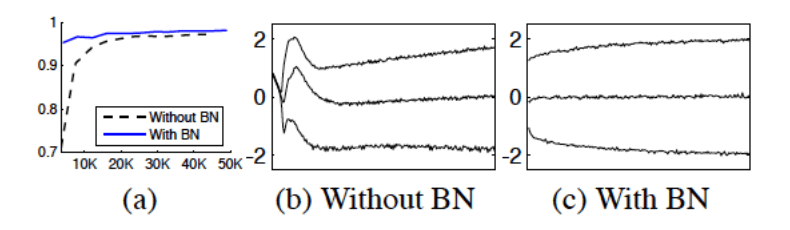
\includegraphics[width=0.7\linewidth]{bn}}
%\caption{Ошибка от эпохи обучения с bn и без него (a); изменение распределения от эпохи обучения без bn (b) и с ним (c)}
%\label{img:bn}
%\end{figure}

%Постановка задачи классификации в нейросетях
\subsection{Постановка задачи классификации в нейросетях}

Пусть дана задача классификации на $M$ классов. Пусть $\mathcal{X}$ -- множество значений индивидов $x$, $\mathcal{Y}$ -- множество классов $y$. Имеем неизвестную зависимость
$$
y=f(x), f: \mathcal{X} \to \mathcal{Y}.
$$

Зафиксируем некоторое подмножество из $m$ индивидов $X \subset \mathcal{X}$, для которых значение целевой функции $f(x)$ известно. Тогда получаем задачу классификации с учителем; ищем такую аппроксимирующую функцию $\hat{y}=f^*(x)$, чтобы функционал качества 
$$
Q(f^*, X)=\frac{1}{m}\sum_{x\in X} \mathcal{L}(f^*(x), f(x))
$$
достигал минимума на $X$. В частности, метод минимизации эмпирического риска:
$$
f^*=\arg\min_{f'\in \mathcal{F}} Q(f', X),
$$
где $\mathcal{F}$ -- класс функций, аппроксимирующих целевую функцию $f(x)$.

Для нейронных сетей данная задача решается для параметризованных аппроксиматоров $f^*(x; \theta)$ путем подбора параметров весов:
$$
\min_{\theta} \frac{1}{m}\sum_{x\in X} \mathcal{L}(f^*(x; \theta), f(x)).
$$

При использовании классификатора в таком виде можем строить только линейные аппроксиматоры; для аппроксимации произвольных функций  вводятся дополнительные слои с нелинейным переходом между ними -- функцией активации $\sigma(.)$. При этом на вход следующих слоев подается выход из предыдущих.

%Особенности при применении к изображениям

При применении данной задачи к изображениям обнаруживается ряд особенностей, позволяющих обособить эту задачу от других:

\begin{itemize}

\item локальная скоррелированость пикселей: как правило, соседние пиксели имеют примерно одинаковую интенсивность;
\item распределенность признака: один пиксель практически не несет в себе информации, признак на изображении -- это совокупность пикселей (иногда на разных каналах);
\item возможные трансформации детектируемых шаблонов: поворот, масштабирование, смещение (например, слишком яркое освещение), перекрытие другими предметами сцены и др.

\end{itemize}

Эти и другие особенности позволили выделить задачи распознавания изображений в отдельный класс задач, и сформировать набор алгоритмов для их решения. Основными идеями, уникальными для этого класса, является применение сверточных и субдискретизационных (pooling) слоев.

%Свертка
\subsection{Свертка}

Свертка помогает выделить признаки из совокупности пикселей. Общая формула свертки функций $f, w$ по области $D$:
$$
(f*w)(x)=\int_D f(y)w(x-y)dy=\int_D f(x-y)w(y)dy;
$$

Например, пусть $f:Z \times Z \to R^K, w: D \times D \to R^K, D = 1..d$ (свертка изображения по ядру $w$ размером $d \times d$ и глубины каналов $K$):
$$
(f*w)(i,j)=\frac{1}{Kd^2}\sum_{k=1}^K \sum_{t,n=1}^d f_k(i-t, j-n) w_k(t,n).
$$

Используем свертку как инструмент выделения локальных особенностей (с учетом специфичности входных данных).

% http://deeplearning.net/tutorial/lenet.html
\begin{definition}[Feature map (activation map)]
Пусть на вход нейросети подается изображение размером $M \times N$. Обозначим его как отображение $x: Z \times Z \to R^3$.
Введем ядро свертки, представляющее собой набор весов $W: Z \times Z \to R^3$. Рассмотрим следующее отображение:
$$
f(i, j): Z \times Z \to R;
$$
$$
f(i, j) = \sigma((W*x)(i, j) + b);
$$
где $b$ --- некоторое смещение, $\sigma$ --- нелинейная функция. Вектор из таких отображений, построенный на разных ядрах $W_k$ и смещениях $b_k$ называется feature map.
\end{definition}
При этом в приведенном примере вход $x$ это тоже feature map глубины 3.

Вместе с весовыми функциями $W_k$ и смещениями $b_k$ они составляют \textbf{сверточный слой}. При этом глубина ядер должна быть равна глубине входа, количество ядер --- количеству желаемых признаков на выходе (глубине входа следующего слоя).

Таким образом, сверточный слой $s$ принимает на вход трехмерную feature map размерностью $N^{(s-1)} \times N^{(s-1)} \times K^{(s-1)}$, производит новую feature map размерностью $N^{(s)} \times N^{(s)} \times K^{(s)}$ посредством $K^{(s)}$ ядер размерностью $d^{(s)} \times d^{(s)} \times K^{(s-1)}$ и $K^{(s)}$ скалярных смещений. Глубина ядер должна быть равна глубине входа, количество ядер --- количеству желаемых признаков на выходе (глубине входа следующего слоя). Подавая на вход различные изображения и обучая сеть при помощи back propagation, мы получим, что задача сведется к оптимизации ядер $W_k$ и смещений $b_k$. Использование свертки позволяет формировать feature maps для выделения признаков из группы соседних индивидов, а не только одного.

%Нелинейность: максимум (ReLU)
\subsection{Функция активации ReLU}

В качестве функции активации в сверточных сетях ниболее часто применяется Rectifier linear unit (ReLU):
$$
f(x)=\max(x, 0).
$$
Гладкая аппроксимация -- softplus:
$$
f(x)=\ln(1+e^x).
$$

\textit{Плюсы:} очень простая производная: $(max(0, x))'=\gamma(x>0)$; нет проблемы vanishing gradient для больших значений на выходе.

\textit{Минусы:} проблема <<мертвых нейронов>>: при достижении нейроном отрицательного выхода градиент становится нулевым, и обучения больше не происходит. Вариант решения проблемы: заменить нулевой отклик на некоторое малое значение. Различные модификации ReLU для решения проблемы <<мертвых нейронов>>:
\begin{itemize}
\item Leaky ReLU ($\epsilon > 0$ -- входной параметр): 
$$
f(x)=
\begin{cases}
x, & x \ge 0, \\
\epsilon x & x < 0.
\end{cases}
$$

\item Shifted ReLU ($\alpha>0$ -- входной параметр): 
$$
f(x)=\max(x, 0) - \alpha.
$$

\item Exponential ReLU (ELU) (a -- обучаемый параметр):
$$
f(x)=
\begin{cases}
x, & x \ge 0, \\
a(e^x-1) & x < 0.
\end{cases}
$$

\end{itemize}

Известно, что ELU обладает большей точностью, чем ReLU, что достигается за счет уменьшения эффекта ковариационного сдвига.
% https://arxiv.org/pdf/1511.07289.pdf

На рисунке~\ref{img:elu} показывается общий график для разных функций активации.

\begin{figure}[h]
\center{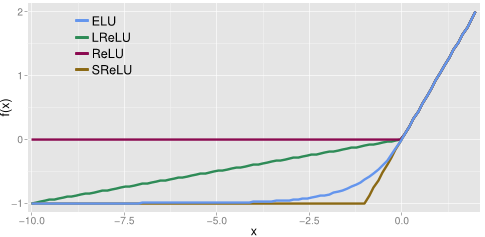
\includegraphics[width=0.7\linewidth]{elu}}
\caption{График разных функций активаций}
\label{img:elu}
\end{figure}

%Пулинг
\subsection{Субдискретизация (Pooling)}

Слой субдискретизации представляет собой нелинейное уплотнение карты признаков, при этом группа пикселей уплотняется до одного пикселя, проходя нелинейное преобразование. Наиболее употребительна при этом функция максимума:
$$
maxpool(x)(i, j)=\max\left(\left\{x(i+t,j+n)\right\}_{t,n=1}^{d}\right),
$$
где $d \times d$ -- размер ядра пулинга. Проходит аналогично свертке по всем координатам входа, но не агрегирует признаки между собой (т.е. двумерна, в отличие от трехмерной свертки).

Операция пулинга позволяет существенно уменьшить пространственный объём изображения. Пулинг интерпретируется так: если на предыдущей операции свёртки уже были выявлены некоторые признаки, то для дальнейшей обработки настолько подробное изображение уже не нужно, и оно уплотняется до менее подробного. Слой пулинга, как правило, вставляется между слоев свёртки.

Кроме max-pooling можно использовать другие нелинейные функции; однако max-pooling считается наиболее удачным для извлечения признаков.

%data augmentation
\subsection{DropOut, Data augmentation}

Две общие техники, представляющие собой способ работы с данными с учетом специфичности:

\begin{definition}{Data augmentation}
(увеличение данных) это техника расширения пространства обучающих индивидов (изображений) путем применения аффинных преобразований и некоторых специфических приемов, например генерация изображений. Например, поворот изображения на некоторый угол, изменение размера изображения и др.
\end{definition}

% https://www.cs.toronto.edu/~hinton/absps/JMLRdropout.pdf
\begin{definition}{DropOut}
--- техника для регуляризации обычной сети путем введения модифицированной модели нейрона: теперь каждый нейрон имеет некоторую вероятность $p$ не участвовать в следующей эпохе обучения сети. Вероятность $p$ является внешним параметром, общим для всех нейронов. При этом в рабочем режиме нейросеть использует все нейроны, т.е. метод применяется только на период обучения. 
\end{definition}

В некотором смысле данная техника эквивалентна обучению множества нейросетей и усреднению результата. Как правило, данную технику не использую в сверточных слоях, однако она может быть полезна в полносвязном слое.

% LeNet, AlexNet
\subsection{LeNet, AlexNet}

Классические архитектуры нейросетей представляют собой несколько сверточных слоев, соединенных последовательно, с постепенным уменьшением размера ядра свертки и чередующимися слоями пулинга. Как правило, свертки используются небольшого размера, из-за затратности их вычисления. Классическими представителями данных архитектур являются сети LeNet и AlexNet.

% http://yann.lecun.com/exdb/publis/pdf/lecun-01a.pdf
Первой полноценной описанной сверточной сетью для изображений стала сеть LeNet (60 тыс. параметров) Она использует тактику постепенного наращивания количества признаков в feature map за счет уменьшения ее размерности (<<воронка>>). На выходе у сверточной части сети находится несколько полносвязных слоев (рис.~\ref{img:lenet}).

\begin{figure}[h]
\center{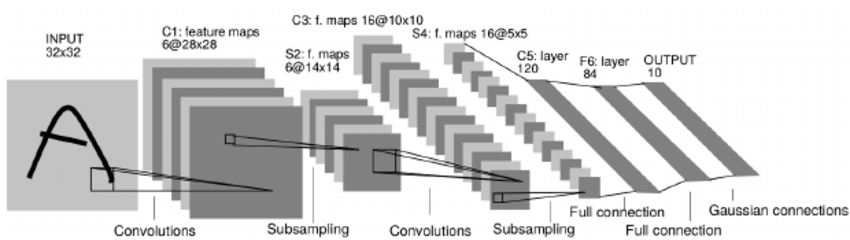
\includegraphics[width=1\linewidth]{lenet}}
\caption{Архитектура LeNet}
\label{img:lenet}
\end{figure}

Уменьшение размерности данных происходит двумя способами: увеличением смещения при перемещении окна свертки и добавлением слоя субдискретизации.

Архитектура AlexNet почти не отличается от архитектуры LeNet (рис.~\ref{img:alexnet}). Имеет 5 сверточных слоев и 3 полносвязных с softmax на 1000 классов на выходе. Она примечательна тем, что это первая сверточная сеть с большим количеством нейронов, использовавшая для обучения два GPU. Параметры: 650 тыс. нейронов, 60 млн. обучаемых параметров, 630 млн связей; функция активации ReLU, 
DropOut с $p=0.5$ на полносвязных слоях; data augmentation.

В данных архитектурах подавляющее большинство обучаемых параметров приходится на полносвязные части. Так, для архитектуры LeNet из 60 тыс. параметров только около 3 тыс. используются на сверточном слое; для AlexNet это 4 млн. из 60 млн. При этом свертка вообще не рассматривается как классификатор, она выступает только лишь как средство выделения признаков.

\begin{figure}[h]
\center{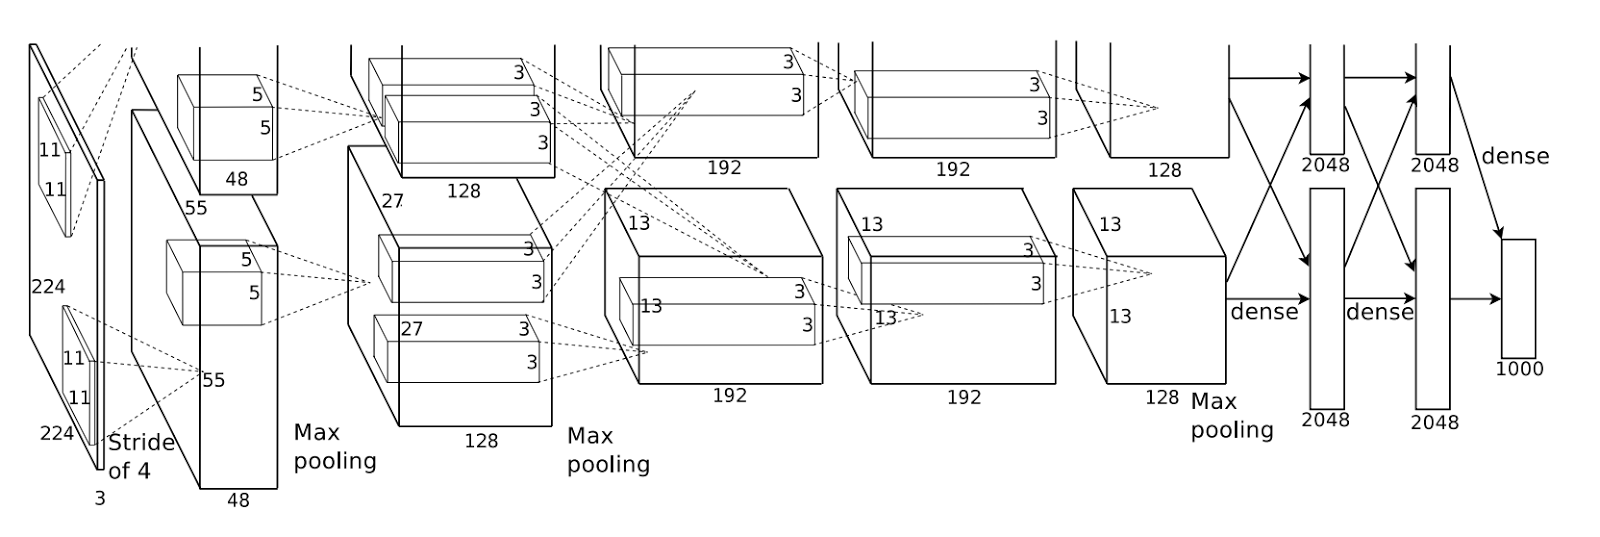
\includegraphics[width=1\linewidth]{alexnet}}
\caption{Архитектура AlexNet}
\label{img:alexnet}
\end{figure}

% Свертка 1х1
% https://arxiv.org/pdf/1312.4400v3.pdf
\subsection{Свертка 1х1}

Пусть $f(i,j) : Z \times Z \to R^K$ -- сверточный слой нейросети с feature map глубиной $K$ признаков; $x(i, j)$ -- вход. Имеем линейное преобразование:
$$
f(i,j)=\sigma((W*x)(i,j) + b).
$$

Оно хорошо представляет данные в случае линейной разделимости признаков. Задача: заменить линейный классификатор более универсальным. В качестве замены линейной модели было предложено использовать обычную многослойную нейронную сеть как особый слой. Схема работы такого слоя следующая:
\begin{gather*}
f_k^{(1)}(i,j)=\sigma(W_k^{(1)} x(i,j) + b_k^{(1)}), \\
... \\
f_k^{(n)}(i,j)=\sigma(W_k^{(n)} f_k^{(n-1)}(i,j) + b_k^{(n)}).
\end{gather*}

Имеем обучаемую функцию c $\sum_{i=1}^n W_k^{(i)}$ весами, принимающую на вход $x(i, j)$ и отдающую $f(i, j) \to R^K$, где $K$ -- количество нейронов на выходном слое перцептрона. 

Выяснилось, что использование при этом $n=1$ позволяет почти произвольным образом менять глубину feature map путем малозатратных вычислений. Это замечание сделало данную модель крайне популярной, так как она способна агрегировать скоррелированные признаки как обычный линейный кассификатор. Эту модель удобно рассматривать в виде свертки $1 \times 1$, чем она по сути и является.

В связи с этим происходит переосмысление взгляда на сверточные слои: это не просто механизмы извлечения признаков для полносвязных слоев в конце, но тоже дискриминаторы.

% Inception
\subsection{Inception (GoogLeNet)}

В архитектуре LeNet и AlexNet есть входной параметр размера ядра свертки конкретного слоя. Если для неглубоких сетей эти параметры можно подбирать, то с ростом глубины сети хотелось бы научиться автоматизировать его выбор (например, сверточные нейросети последних поколений имеют количество слоев $>1000$). Возникает идея: ввести такую модель, чтобы слой сам мог решать, какой размер ядра ему нужен.

Примером такой модели стала архитектура Inception (рис.~\ref{img:inception_layer}). Основное предположение заключается в следующем: если разделить вход на несколько неглубоких feature map при помощи ядер $1 \times 1$ и выделить признаки на ядрах разного размера, то такая архитектура сможет собрать максимальное количество признаков для данной feature map. На выходе выделенные feature map объединяются простой конкатенацией в одну общую карту и передаются следующему слою.

Общая схема для модуля Inception: выходной слой агрегирует преобразования на ядрах размера $n \times n$, $(2n-1) \times (2n-1)$ и пулинге размера $n$. Слои $1 \times 1$ используются для преобразования глубины feature map для ускорения вычислений.

\begin{figure}[h]
\center{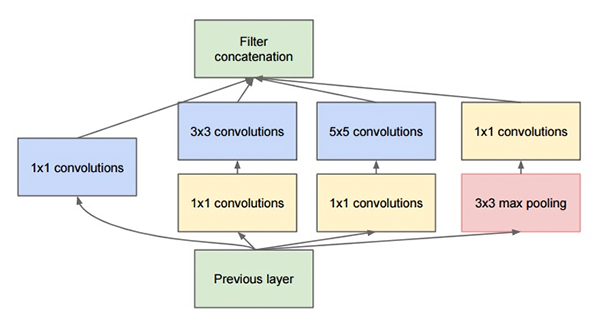
\includegraphics[width=0.4\linewidth]{inception_layer}}
\caption{Архитектура блока Inception}
\label{img:inception_layer}
\end{figure}

Первой сетью, активно внедрившей данную идею, стала сеть GoogLeNet. Ее архитектура представлена на рисунке~\ref{img:googlenet}.

В начале сеть плавно набирает достаточное количество признаков, затем используется ряд блоков Inception. В конце используется полносвязный слой. Еще одной новой идеей в данной архитектуре стало ответвление промежуточных вспомогательных классификаторов, использующихся только при обучени сети. Изначально их роль состояла в том, чтобы помочь сети обучаться быстрее и точнее, впоследствии выяснилось, что единственный полезный эффект от таких включений -- дополнительная регуляризация.

\begin{figure}[h]
\center{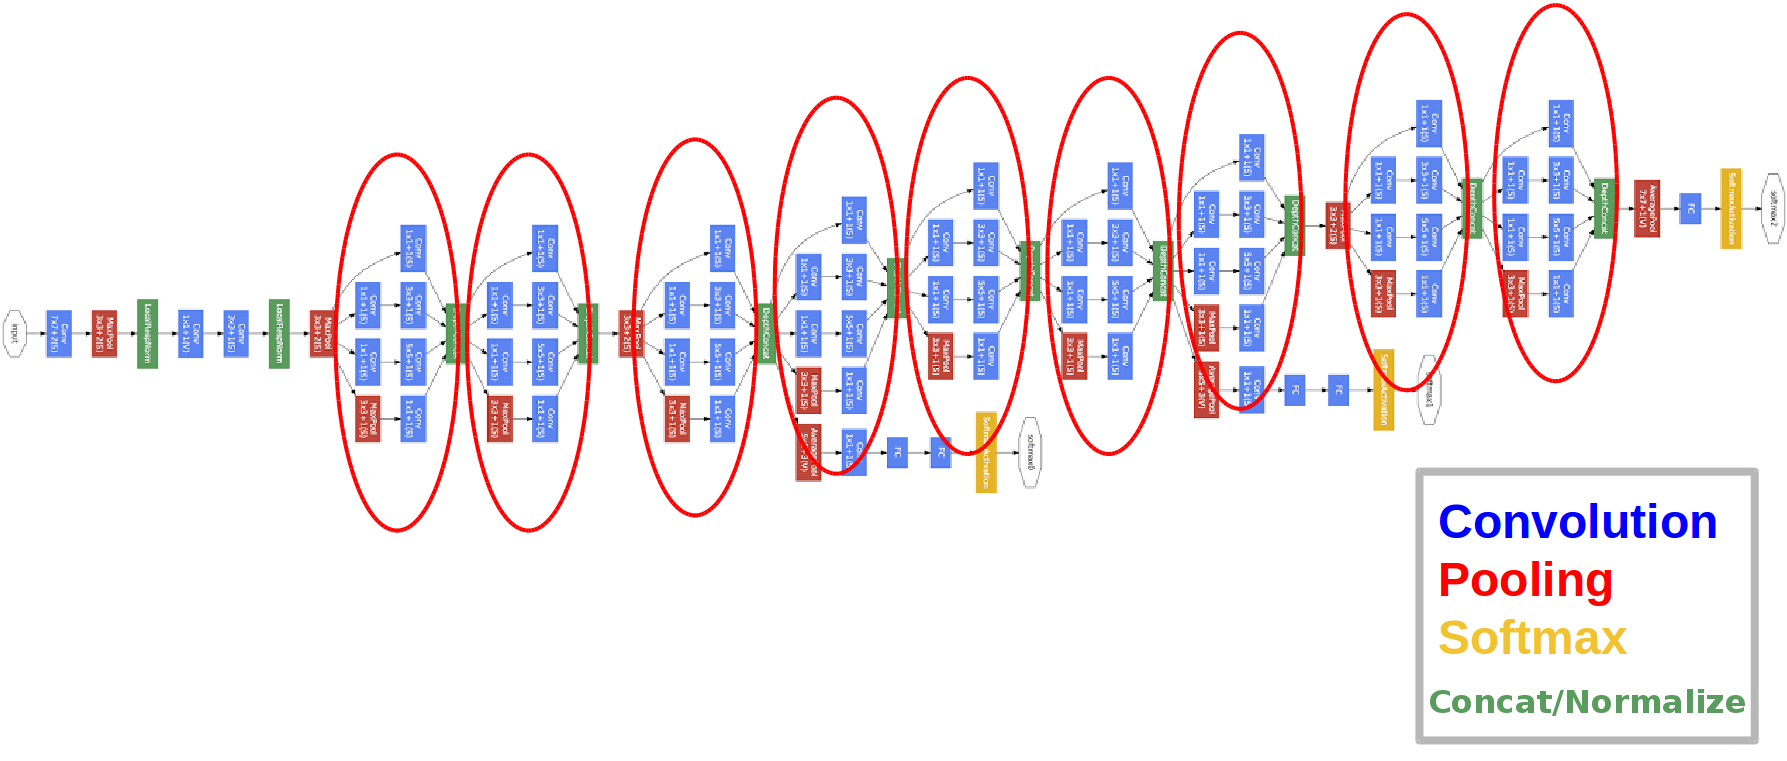
\includegraphics[width=1\linewidth]{googlenet}}
\caption{Архитектура GoogLeNet}
\label{img:googlenet}
\end{figure}

Параметры модели: 9 блоков Inception, 2 вспомогательных классификатора. Вход: изображение $224 \times 224$, выход 1000 классов.

% Ковариационный сдвиг
% http://citeseerx.ist.psu.edu/viewdoc/download?doi=10.1.1.370.4921&rep=rep1&type=pdf
\subsection{Внутренний ковариационный сдвиг (internal covariate shift)}


Рассмотрим общую задачу классификации. Имеем набор индивидов $x$ и некоторый целевой признак $y$. Хотим получить оценку условной плотности $q(y|x)$ по известным парам $(x, y)$, через параметрическую модель: 
$$
q(x|y)=p(y|x; \theta).
$$

По некоторой предоставленной выборке $(X, Y)$ оптимизируем $\hat{\theta}$ при помощи функционала качества:
$$
\hat{\theta}=\arg \min Q(Y, \Expect[Y|X; \theta]).
$$

При этом $|\hat{\theta} - \theta| > 0$, а следовательно $p(x; \hat{\theta}) \ne p(x; \theta)$. 

Данная модель применима к одному нейрону в многослойной нейросети, со входом $x=f^{(s-1)}$, выходом $y=f^{(s)}$ и весами $\hat{\theta}=W^{(s)}$. Это означает, что при обучении распределение первого слоя ($s=1$) будет стабилизироваться, и плотность $p^{(1)}(y|x; \hat{\theta})$ будет стремиться к $p^{(1)}(y|x; \theta)$. Однако это же означает, что для второго слоя распределение входных данных будет изменяться, возможно значительно; следовательно, для него данное замечание, вообще говоря, недействительно, и его параметры $\hat{\theta}^{(2)}$ могут оцениваться неверно. 

На практике данная проблема хорошо известна под названием <<внутренний ковариационный сдвиг>> (internal covariate shift). Из-за этого, как правило, страдает точность классификации, и значительно страдает скорость обучения. Одним из способов борьбы со сдвигом является стандартизация входных данных; в 2015 году было предложено решение данной проблемы при помощи алгоритма batch normalization.

% batch normalization
% http://proceedings.mlr.press/v37/ioffe15.pdf
\subsection{Batch normalization}

Пусть:
\begin{itemize}
\item $f(i,j) : Z \times Z \to R^K$ --- feature map на входе слоя глубины $K$ и размерности $N \times M$;
\item $x=x_{i,j} \in R^{K}$ -- индивиды (пиксели).
\end{itemize}

Введем предположение, что $x$ распределены по $K$-мерной плотности распределения $P(x; \Sigma, \mu)$. Вход первого слоя имеет постоянное распределение, вход произвольного слоя изменчив, так как вычисляется на основе предыдущих слоев --- функций с переменными коэффициентами. Для дальнейшего рассмотрения зафиксируем распределение $P$, однако учтем, что оно может меняться в процессе обучения. 

Пусть $X \in R^{K \times MN}$ --- набор всех индивидов на данной feature map $f$. Тогда $\hat{\Sigma}$ --- оценка матрицы ковариации входа, $\hat{\mu}$ --- оценка смещения входа. Стандартизацию входа, как и всякую трансформацию исходных данных, нужно будет учитывать при обратном проходе backprop: необходимо уметь вычислять на каждом шаге следующий якобиан:
$$
\frac{\partial}{\partial x} \hat{\Sigma}^{-1/2}(x-\hat{\mu}).
$$

Это очень дорого и неэффективно, потому вводится предположение о независимости компонент распределения $P(x; \Sigma, \mu)$, т.е. $\Sigma$ диагональная, и имеем вектор из дисперсий $\sigma_k^2$. (Это предположение как правило не выполняется, но все равно позволяет получить более высокую скорость обучения). В итоге имеем покомпонентно стандартизированный выход:
$$
\bar{x}_{k, i} = \frac{x_{k, i} - \hat{\mu}_k}{\hat{\sigma}_k}.
$$

Данная операция стандартизирования порождает проблему: мы ограничили область значений исходной feature map $f(i, j)$, что может сказаться на предсказательной способности.

Предположим, что исходная feature-map была оптимальна для построения по ней следующего слоя; тогда стандартизация ухудшит его отклик. Для решения этого авторы вводят возможность тождественного отображения через дополнительные обучаемые параметры scale и shift:
$$
y_{k,i}=\gamma_k \bar{x}_{k,i} + \beta_k.
$$

При $\gamma = \sigma_k$ и $\beta = \mu_k$ получаем тождественное равенство.

Таким образом, если рассматривать исходные параметры смещения и масштаба исходной feature map как случайные, то процедура сводится к удалению этих случайных параметров и замене их на обучаемые.

Запишем в общем виде процесс обучения на нейроне:
$$
f=\sigma((W*x)+b).
$$

В процессе обучения batch normalization добавляется непосредственно перед функцией активации $\sigma(.)$, т.е. действует на $Wx + b$. Проведя несложные подсчеты, можно убедиться, что при исключении $b$ из этой формулы ничего не изменится, так как ее роль принимает на себя $\beta$:
\begin{gather*}
f=\sigma(BN((W*x)+b))\\=
\sigma(\gamma\frac{((W*x)+b)-\hat{\mu}}{\hat{\sigma}}+\beta)\\= 
\sigma\left(\frac{\gamma}{\hat{\sigma}}(W*x)+\left( \frac{\gamma}{\hat{\sigma}}(b-\hat{\mu}) + \beta \right)\right).
\end{gather*}

В таком виде batch normalization был предложен в оригинальной статье.

Возможности инструмента:
\begin{itemize}
\item регуляризация за счет исправления смещения;
\item позволяет использование больших шагов градиента и как следствие ускорение обучения.
\end{itemize}

На рис.~\ref{img:bn} представлены графики из оригинальной статьи по batch normalization. В части (a) показывается ошибка при тестирования сети, обученной с bn и без него. На (b, c) отображены 15-, 50- и 85-квантили распределения одного из входов сети без использования bn (b) и с ним (с). Распределения в исходной сети значительно меняются со временем, как по их среднему значению, так и по дисперсии, что усложняет обучение последующих слоев. Напротив, распределения в сети с использованием bn намного более стабильны.

\begin{figure}[h]
\center{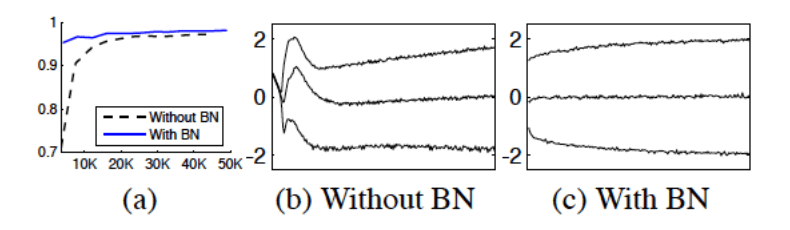
\includegraphics[width=1\linewidth]{bn}}
\caption{Ошибка от эпохи обучения с bn и без него (a); изменение распределения от эпохи обучения без bn (b) и с ним (c)}
\label{img:bn}
\end{figure}


\subsection{ResNet, Inception ResNet}
%проблема: взрыв и затухание градиента с ростом числа слоев
%ResNet, Inception ResNet
% degradation problem

С ростом числа слоев в нейросетях возникает проблема \textbf{деградации сети}: при увеличении количества слоев нейросети интуитивно логично ожидать улучшения качества предсказания, что на практике оказывается неверно. Предположения о переподгонке не оправдываются, так как с ростом числа слоев растет ошибка даже на тренировочном наборе данных. Предполагаемые причины: затухание градиента, экспоненциальное увеличение времени обучения с ростом числа слоев.

Задача: получить такую архитектуру, которая позволяла бы наращивать число слоев и не ухудшать предсказательную способность на обучающей выборке. Решение сходно с идеей бустинга: обучение на остатках. Отсюда название архитектуры таких сетей --- residual network (ResNet).

Для решения данной проблемы используется архитектура с прямым подключением входа к каждому сверточному слою (рис.~\ref{img:resnet}). Пусть исходная задача представляется в виде аппроксимации некоторой сложной функции $\mathcal{H}(x)$ сверточной сетью $\mathcal{F}(x)$; исходно задача записывалась бы в виде $\mathcal{H}(x)=\mathcal{F}(x)$, однако в данном случае предлагается использовать модель вида $\mathcal{H}(x)=\mathcal{F}(x)+x$.

\begin{figure}[h]
\center{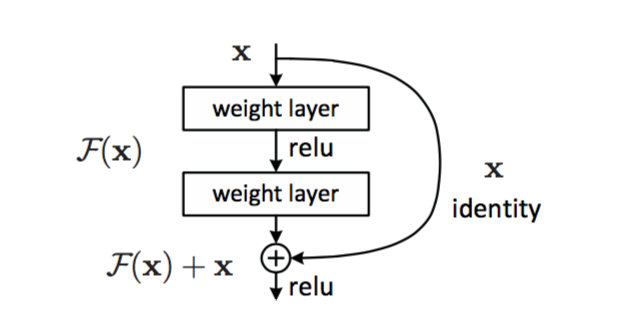
\includegraphics[width=0.4\linewidth]{resnet}}
\caption{Модель слоя с подключением ко входу}
\label{img:resnet}
\end{figure}

Это простое расширение архитектуры позволило увеличить максимальную глубину сетей в десятки раз, при этом добавление нового слоя как минимум не ухудшает результат предсказания.

На рисунке~\ref{img:IncResNet_v2} показана архитектура сети Inception ResNet v2.

\begin{figure}[h]
\center{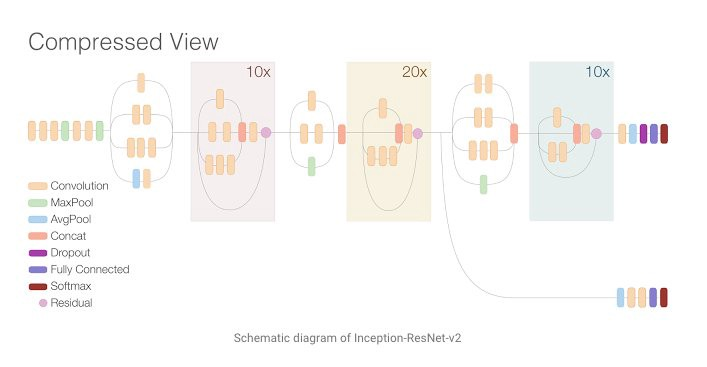
\includegraphics[width=1\linewidth]{IncResNet_v2}}
\caption{Архитектура сети Inception ResNet v2}
\label{img:IncResNet_v2}
\end{figure}

Сети такого вида можно представить в виде ансамблей, способных работать даже при отключении некоторых слоев. При этом используются слои с малой глубиной feature map, как <<слабые классификаторы>> в бустинге, что помогает увеличить скорость обучения. Подключение входа представляется в виде суммирования с выходом предыдущего слоя; это обязует слои быть одной размерности по всем измерениям.

% https://arxiv.org/pdf/1608.06993.pdf
\subsection{DenseNet}

В августе 2017 года вышла статья, в которой архитектура ResNet была немного изменена. А именно, если в исходном алгоритме использовалось подключение в виде суммирования:
$$
\mathcal{H}(x)=\mathcal{F}(x)+x,
$$

то в данном случае авторы предложили использовать конкатенацию, как в Inception. Это меняет модель так, что теперь на вход к текущему слою подаются выходы всех предыдущих:
$$
x^{(s)}=\mathcal{F}(x^{(1)}, x^{(2)}, ..., x^{(s-1)}),
$$

При этом глубина последнего слоя равна
$$
K^{(M)}=K^{(0)} + \sum_{s=1}^M K^{(s)},
$$
где $K^{(0)}$ --- глубина входного слоя, $K^{(s)}$ --- глубина слоя $s$. Это делается для того, чтобы не переусложнять модель. Предлагается использовать простейшие сверточные слои небольшой глубины и размера ядра ($3 \times 3$). Пример блока Dense для трех слоев показан на рисунке~\ref{img:densenet0}.

\begin{figure}[h]
\center{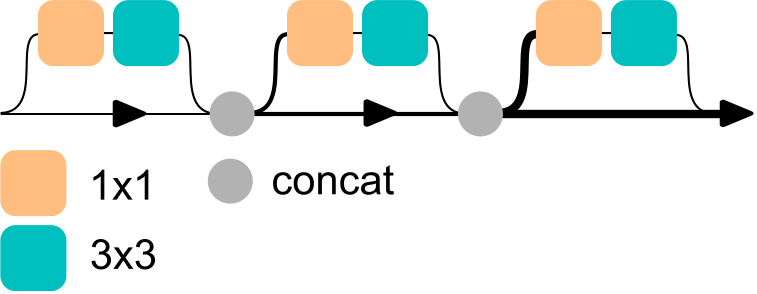
\includegraphics[width=0.5\linewidth]{densenet0}}
\caption{Архитектура блока Dense}
\label{img:densenet0}
\end{figure}

Также, аналогично архитектуре Inception ResNet, используются блоки из слоев данной модели, разделенные слоями с пулингом для уменьшения размерности карты признаков. 

Архитектура сети DenseNet в качестве единичного слоя использует слой с уплотнением признаков $1 \times 1$, плюс сверточный слой $3 \times 3$. Используется ReLU, регуляризация: BN. 

\begin{figure}[h]
\center{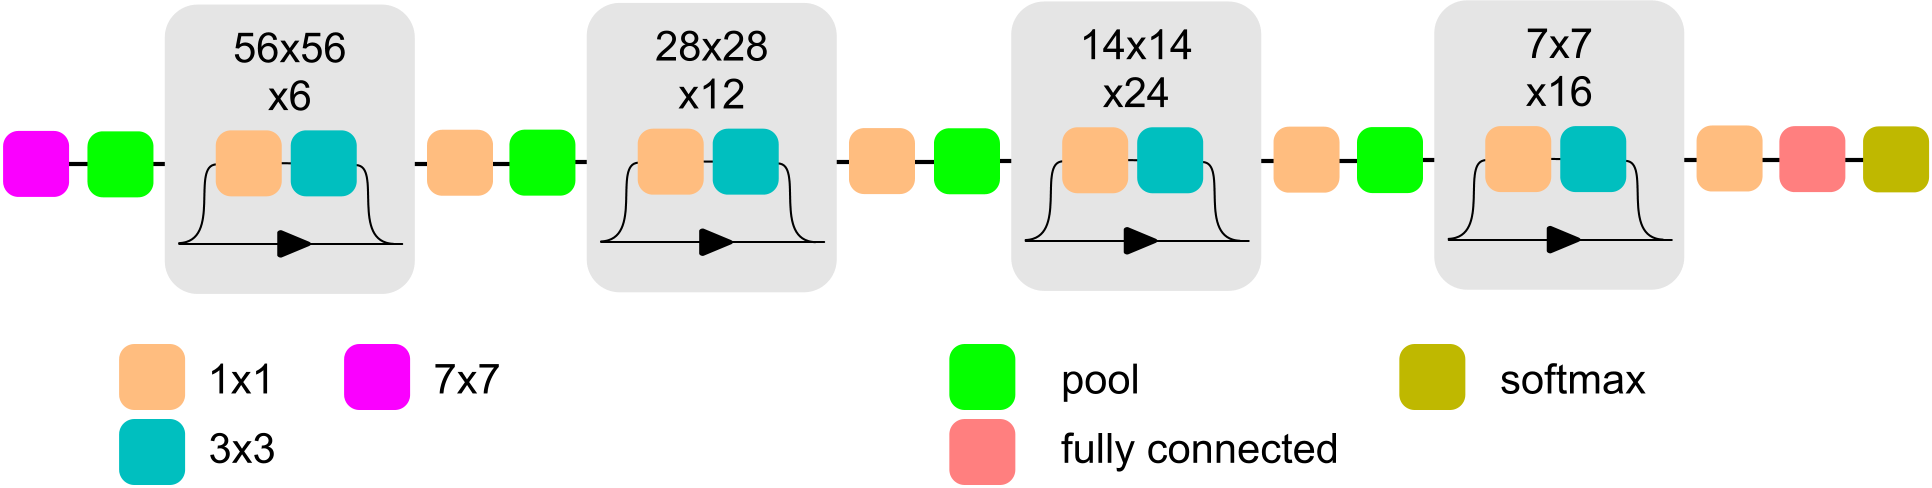
\includegraphics[width=0.8\linewidth]{densenet1}}
\caption{Архитектура сети DenseNet}
\label{img:densenet1}
\end{figure}

Сеть имеет 4 <<Dense>> блока: на 6, 12, 24 и 16 слоев; между ними переходные слои (<<transition layer>>) для уменьшения размерности. Вход $112 \times 112$, выход 1000 классов через полносвязный слой. Результаты показывают, что данная архитектура быстрее обучается и точнее работает по сравнению с ResNet с аналогичным количеством параметров.

\end{document}